\documentclass[times, utf8, diplomski, numeric]{fer}
\usepackage{booktabs}
\usepackage{courier}
\graphicspath{ {./slike/} }
\usepackage[parfill]{parskip}

% dodano za prekidanje URL-ova na / i -
\usepackage{url}
\def\UrlBreaks{\do\/\do-}

\begin{document}

% TODO: Navedite broj rada.
\thesisnumber{000}

% TODO: Navedite naslov rada.
\title{Proširivi sustav za stvaranje CTF zadataka specifičnih za sustave upravljanja i
zabave u automobilima}

% TODO: Navedite vaše ime i prezime.
\author{Lovro Grgurić Mileusnić}

\maketitle

% Ispis stranice s napomenom o umetanju izvornika rada. Uklonite naredbu \izvornik ako želite izbaciti tu stranicu.
\izvornik

% Dodavanje zahvale ili prazne stranice. Ako ne želite dodati zahvalu, naredbu ostavite radi prazne stranice.
\zahvala{}

\tableofcontents

\chapter{Uvod}
Današnji automobili i ostala cestovna vozila značajno se razlikuju od njihovih prvih inačica, iako im glavna namjena ostala ista. Pojavom i širom primjenom elektronike, automobili više nisu samo mehanički strojevi, već sadrže određen broj međusobno povezanih elektroničkih upravljačkih jedinica (engl. \textit{electronic control unit}, ECU) \cite{koscher2010}. Elektroničke upravljačke jedinice svojom međusobnom suradnjom omogućavaju sigurno upravljanje vozilom, ali i dodatne funkcionalnosti poput klimatizacije te sustava za informacije i zabavu (engl. \textit{in-vehicle infotainment}). Većina komunikacije između elektroničkih upravljačkih jedinica odvija se putem protokola poput \textit{Controller Area Network} (CAN) protokola i pripadajućih sabirnica. Prvotno namijenjen za primjenu u automobilima, CAN ima svojstva prikladna za komunikaciju u stvarnom vremenu (engl. \textit{real time}), kao i sposobnosti detektiranja grešaka i propuštanja poruka višeg prioriteta \cite{canopen1}. Međutim, iako ga specifikacija druge inačice CAN protokola, CAN 2.0, opisuje kao protokol s visokom razinom sigurnosti, ni ta niti originalna specifikacija ne razmatraju osiguravanje osnovnih sigurnosnih svojstava povjerljivosti, integriteta i dostupnosti (engl. \textit{confidentiality, integrity, availability}, CIA) \cite{bosch1991, canislabs1}. Zbog drastične prirode posljedica koje bi neispravan rad sustava automobila mogao imati na vozača i njegove suputnike te ostale sudionike prometa, pri inženjeringu sustava automobila uvijek je bila pridodana posebna pažnja njihovoj funkcionalnoj sigurnosti (engl. \textit{safety}) i ispravnosti, ali ne nužno i kibernetičkoj sigurnosti \cite{koscher2010}. Zbog tadašnje zatvorenosti komunikacije ovih sustava, za potencijalnog napadača nije postojala površina (engl. attack surface) koju bi mogao iskoristiti bez fizičkog pristupa CAN sabirnici.

Interne mreže današnjih vozila kao i programska podrška njihovih sustava znatno su kompleksnije i povezanije s vanjskim svijetom \cite{huq2020driving}. Mnogi novi modeli automobila su opremljeni SIM karticama odnosno mogućnošću povezivanja na mobilnu mrežu u svrhu komunikacije sa servisima proizvođača u oblaku (engl. cloud services) i mobilnim aplikacijama koje omogućuju udaljeno upravljanje vozilom. Uz nevedeno, mobilna mreža koristi se i u svrhu preuzimanja ažuriranja (engl. \textit{Over-The-Air updates}, OTA) za sustave zabave, ali i za kritične elektroničke upravljačke jedinice. \textit{Bluetooth} tehnologija najčešće se koristi za povezivanje mobilnog telefona sa sustavom zabave kako bi se omogućilo pozivanje i reprodukcija glazbe. U svrhu bolje integracije mobilnih telefona u sustav zabave, mnogi proizvođači podržavaju platforme poput \textit{Android Auto} ili \textit{Apple Carplay}, kojima se sustav zabave proširuje mogućnostima preuzimanja i pokretanja raznovrsnih aplikacija iz izvora treće strane. Vozila opremljena mrežnim karticama s mogućnošću stvaranja i korištenja Wi-Fi bežičnih pristupnih točaka, mogu dijeliti pristup mobilnoj mreži koji ostvaruju s prethodno navedenim SIM karticama ili povezivati se na pristupne točke korisnika u svrhu preuzimanja OTA ažuriranja ili aplikacija. Za skoro svaku od navedenih funkcionalnosti istraživači automobilske sigurnosti pokazali su mogućnost njihvog iskorištavanja i ulančavanja otkrivenih ranjivosti u svrhu neautoriziranog pristupa i postizanja kontrole nad sustavima zabave, ali i kritičnim sustavima upravljanja automobila \cite{nie2017free, nie2018over, cai20190, tencent2018bmw, miller2015remote, curry2023web}. Nadalje, već u izvješću o stanju automobilske sigurnosti tvrtke \textit{Upstream Security} iz 2019. godine, predviđa se da će sva nova vozila proizvedena u 2025. godini imati navedene funkcionalnosti, ali i da će podržavati komunikaciju među vozilima (engl. \textit{Vehicle-to-Vehicle, V2V}) i komunikaciju vozila s infrastrukturom (engl. \textit{Vehicle-to-Infrastructure, V2I}), dodatno povećavajući dostupnu površinu napada \cite{upstream2019report}.

Nagli rast povezanosti i kompleksnosti sustava vozila stvara potrebu za obrazovanjem određenog broja stručnjaka i inženjera koji će testirati i osiguravati kvalitetniju kibernetičku sigurnost tih sustava, od razine sklopovlja do \textit{backend} servisa te V2V i V2I komunikacije. Osim formalnih sustava obrazovanja, popularan format za edukaciju stručnjaka kibernetičke sigurnosti su i \textit{Capture the Flag} (CTF) zadaci. Međutim, u \cite{vsvabensky2021cybersecurity} autori ističu da se u analiziranom uzorku od 12 952 \textit{Capture the Flag} zadataka, zadaci klasificirani u područje sigurnosti komponenti (engl. \textit{component security}) čine tek 8,19\%, što je 6. najmanji udio od ukupno 8 analiziranih područja znanja. Većina današnjih \textit{Capture the Flag} zadataka spada u razvijenije i poznatije grane kibernetičke sigurnosti poput \textit{web} sigurnosti, sigurnosti operacijskih sustava i aplikacija te sigurnosti oblaka (engl. \textit{cloud security})\cite{prinetto2020hardware}. U svrhu edukacije sigurnosnih stručnjaka u području kibernetičke sigurnosti u automobilskoj industriji potrebno je napraviti proširivi sustav koji će služiti kao temelj za stvaranje \textit{Capture the Flag} zadataka koji sadrže specifičnosti sustava u automobilima.

Rad je strukturiran kroz 6 poglavlja. U prvom poglavlju nakon uvoda, odnosno drugom poglavlju cjelokupnog rada, napravljen je pregled protokola te arhitekture modernog automobila. Kroz ovo poglavlje bit će opisani protokoli korišteni u današnjim automobilima kao i sustavi koje povezuju, čime se postavlja teoretska i tehnička podloga za razumijevanje napada na iste, opisanih u trećem poglavlju. U četvrtom poglavlju razmatraju se postojeći sustavi za obuku stručnjaka sigurnosti u grani sigurnosti automobila, ali i u ostalim granama sigurnosti te je definiran popis poželjnih svojstava takvog sustava. U petom poglavlju opisana je implementacija proširivog sustava za stvaranje \textit{Capture the Flag} zadataka specifičnih za sustave upravljanja i zabave u automobilima. Naposljetku, u zaključku su opisani konačan rezultat, prednosti i nedostatci implementiranog sustava te moguća unaprjeđenja i smjernice za daljnji razvoj.

\chapter{Sustavi i protokoli modernih automobila}
Kao temelj za razumijevanje iskoristivih površina i mogućih vektora napada na sustave automobila, kroz ovo poglavlje opisana je električna i elektronička arhitektura modernog automobila (engl. \textit{Electrical/Electronic} architecture). Opisani su i protokoli specifični za automobile kroz više slojeva OSI modela.
\section{E/E arhitektura modernog automobila}
E/E arhitektura obuhvaća elektroničke komponente, električko ožičenje, tehnologije umrežvanja i programsku podršku jednog automobila \cite{nasser2023automotive}. Prema \cite{nasser2023automotive, koscher2010, knight2020hacking, huq2020driving, aliwa2021cyberattacks}, sustavi vozila dijele se prema funkciji u domene:

\begin{itemize}
    \item pogonskog sklopa (engl. \textit{powertrain})
    \item šasije (engl. \textit{chassis})
    \item kabine (engl. \textit{interior cabin} ili \textit{body})
    \bigskip
    \item zabave i povezivosti (engl. \textit{infotainment and connectivity})
\end{itemize}

Iako se sustavi mogu prema funkciji podijeliti u navedene 4 domene, domene nužno ne određuju topologiju mreže automobila.

Domene pogonskog sklopa, šasije i kabine sadrže ECU-ove koji najviše utječu na fizičko stanje automobila te je njihova komunikacija većinom ograničena na internu mrežu automobila. Domena informacija, zabave i povezivosti sadrži sustave koji pružaju dodatne informacije i sadržaje vozaču i putnicima te vrše komunikaciju i s okolinom automobila, primjerice s \textit{backend} servisima, mobilnim uređajima i aplikacijama. Stoga je domena informacija, zabave i povezivosti obrađena u zasebnom potpoglavlju.   
\subsection{Domene pogonskog sklopa, šasije i kabine}
Elektroničke upravljačke jedinice odnosno ECU-ovi, pripadaju domenama pogonskog sklopa, šasije i unutarnje kabine te služe za koordiniranje i upravljanje većinom funkcija automobila. ECU-ovi detektiraju trenutne operativne uvjete pomoću senzora, procesuiraju ih i aktiviraju aktuatore \cite{bosch2022handbook}. Sklopovlje ECU-a najčešće se nalazi u zatvorenom zaštitnom kućištu s izloženim priključcima za spajanje na ostatak mreže automobila, senzore i aktuatore. Sklopovlje je najčešće tiskana pločica na kojoj se najčešće nalazi integrirani krug za upravljanje snagom (engl. \textit{power management integrated circuit}, PMIC), primopredajnici protokola kojim komuniciraju, memorije te mikrokontroler ili sustav na čipu (engl. \textit{System on a chip}), SoC)\cite{nasser2023automotive}. ECU-ovi ovih domena najčešće zbog \textit{real time} zahtjeva međusobno komuniciraju putem CAN ili FlexRay protokola, gdje specifična topologija mreže ovisi o modelu automobila \cite{bosch2022handbook}.

Domeni pogonskog sklopa pripadaju ECU-ovi koji upravljaju i utječu na funkciju motora i prijenosa, a to su upravljački modul motora (engl. \textit{engine control module}, ECM) i upravljački modul prijenosa (engl. \textit{transmission control module}, TCM). U literaturi se često koriste i nazivi upravljačka jedinica motora (engl. \textit{engine control unit}, ECU), odnosno upravljačka jedinica prijenosa (engl. \textit{transmission control unit}, TCU)\cite{nasser2023automotive, koscher2010}. Često automobili imaju jedan snažniji ECU koji obavlja obje funkcije, upravljanje motorom i upravljanje prijenosom te se takav ECU naziva upravljačkom jedinicom pogonskog sklopa (engl. \textit{powertrain control unit}, PCU) ili upravljačkim modulom pogonskog sklopa (engl. \textit{powertrain control module}, PCM) \cite{bosch2022handbook, ecutesting}. U slučaju vozila na električni pogon, u domeni pogonskog sklopa pripadaju sustav upravljanja baterijom (engl. \textit{battery managment system}, BMS), inverter \engl{inverter} i PCU. Uz navedene, u domenu pogonskog sklopa ulaze i druge upravljačke jedinice koje prikupljaju podatke sa senzora i upravljaju aktuatorima relevantnima pogonskom sklopu. S obzirom na to da navedeni ECU-ovi imaju izravan utjecaj na kretanje automobila, njihovo kompromitiranje može rezultirati fizičkim ozljedama vozača i putnika.

U domenu šasije svrstavaju se sustavi i senzori odgovorni za funkcije zaštite putnika koje zahtijevaju reakciju u stvarnom vremenu poput sustava kočenja, ovjesa i zračnih jastuka. Sukladno tome, kao i u slučaju sustava domene pogonskog sklopa, njihovo ispravno funkcioniranje je iznimno bitno za sigurnost vozača i putnika \cite{nasser2023automotive}. Jedna od upravljačkih jedinica koje pripadaju u domenu šasije je upravljački modul elektroničkog kočenja (engl. \textit{electronic braking control module}, EBCM). EBCM je specijalizirani modul koji upravlja aktivnim sigurnosnim mjerama poput ABS-a (njem. \textit{Antiblockiersystem}), elektroničkom kontrolom stabilnosti (engl. \textit{electronic stability control}, ESC) te automatskog hitnog kočenja (engl. \textit{automated emergency breaking}, AEB). Uz EBCM, u domenu šasije svrstavaju se i napredni sustav za podršku vozaču pri upravljanju vozilom (engl. \textit{Advanced driver-assistance system}, ADAS), koji je sve češće prisutan u novim vozilima \cite{nasser2023automotive}. ADAS je odgovoran za funkcije poput rada tempomata, održavanja razmaka između vozila,  automatskog zadržavanja trenutne prometne trake, automatskog parkiranja te autonomne vožnje \cite{bosch2022handbook}. Domeni šasije pripada i upravljački modul zračnih jastuka (engl. \textit{airbag control module}, ACM) te sustav servo upravljača (engl. \textit{electronic power steering}, EPS). ADAS i EBCM prikupljaju podatke od niza sustava senzora, primjerice od radara za određivanje udaljenost objekata u svrhu aktivacije funkcije AEB, od ultrazvučnih senzora za potrebe sustava automatskog parkiranja te od sustava lidar i video senzora za potrebe autonomne vožnje. 

U domenu kabine spadaju sustavi manje kritičnih funkcija te uključuju sustave grijanja, ventilacije i klimatizacije (engl. \textit{heating, ventilation and air conditioning}, HVAC), pripadajući upravljački modul klimatizacije (engl. \textit{climate control module}, CCM) te ECU-ove za prikupljanje podataka sa senzora sigurnosnih pojasa i sjedala te ECU-ove za upravljanje ambijentalnim osvjetljenjem, prozorima, brisačima i ostalim dijelovima kabine. Uz navedene, kao sigurnosno bitni sustavi, ističu se sustav za ulaz bez ključa (engl. \textit{keyless entry system}, KES) te ECU za upravljanje otključavanjem vrata vozila i pripadajući prijemnik za daljinsko zaključavanje (engl. \textit{remote control door lock receiver}, RCDLR). KES i RCDL sustavi najčešće su iskorištavani sustavi u slučaju krađe vozila, često putem \textit{relay} napada \cite{nasser2023automotive, cbc2020relay}.

\subsection{Domena informacija, zabave i povezivosti}
Suprotno domenama pogona, šasije i kabine, domena informacija, zabave i povezivosti sadrži sustave čije funkcionalnosti većinom nisu visokog prioriteta niti su uvjetovane \textit{real time} zahtjevima. Sustav za informacije i zabavu, odnosno IVI, obuhvaća niz podsustava koji vozaču i putnicima pružaju informacije o stanju vozila i dodatne sadržaje. 

Ploča s instrumentima \engl{instrument cluster}, u mehaničkoj izvedbi ili kao digitalni zaslon, pruža vozaču informacije o brzini vozila, broju obrtaja motora i količini preostalog goriva te stanju pokazivača smjera, tempomata i kvarova kroz određen broj indikatorskih svjetlećih dioda. U digitalnoj izvedbi, ploča s instrumentima može prikazivati i druge korisne informacije, kako vozač ne bi morao skretati pogled na središnji zaslon tijekom vožnje, poput trenutne radio postaje, parking kamere te navigacije \cite{bosch2022handbook, nasser2023automotive}. 

Navigacija se često prikazuje i na središnjem zaslonu u sklopu grafičkog sučelja operacijskog sustava središnje jedinice \engl{head unit}. Središnji zaslon je često osjetljiv na dodir ili je njime moguće upravljati pomoću fizičkih tipki na središnjoj konzoli. Putem grafičkog sučelja vozač i putnici vozila mogu iskoristiti mogućnost povezivanja mobilnog telefona sa sustavom za informacije i zabavu putem \textit{Bluetooth} tehnologije ili USB-a, u svrhu reprodukcije glazbe i telefoniranja.

Noviji modeli automobila podržavaju integraciju s platformama poput \textit{Android Auto} i \textit{Apple Carplay}, koji omogućavaju puno dublju integraciju funkcija mobilnog telefona u sustave informacija i zabave. Povezivanjem telefona s njemu pripadajućom platformom, korisnicima automobila omogućava korištenje aplikacija za navigaciju, reprodukciju glazbe i ostalih multimedija, korištenje \textit{web} preglednika, telefoniranje i razmjenu poruka s njihovog mobilnog uređaja. Omogućavaju i integraciju obavijesti, kalendara te "pametnih" asistenata \cite{androidauto, carplay}.

Primarna funkcija upravljačke jedinice za telematiku (engl. \textit{telematics control unit}, TCU), je omogućavanje povezivosti automobila putem mobilne mreže, \textit{Wi-Fi} i \textit{Bluetooth} tehnologija te prijam GPS signala \cite{nasser2023automotive}. Povezivost putem \textit{Wi-Fi} tehnologije i mobilne mreže koristi se u svrhu transmisije telemetrijskih podataka, preuzimanja OTA ažuriranja te komunikaciju s \textit{backend} servisima proizvođača, ali i u svrhu zaštite putnika pozivanjem hitnih službi u slučaju prometne nesreće.

Operacijski sustav središnje jedinice najčešće je utemeljen na \textit{Linux}, \textit{QNX} i \textit{Android} operacijskim sustavima ili operacijskom sustavu proizvođača (engl. \textit{proprietary} \cite{nasser2023automotive}. Operacijski sustav objedinjuje sve navedene funkcionalnosti te omogućava upravljanje istima putem središnjeg zaslona, konzole i te putem glasa \cite{bosch2022handbook}. Zbog visoke razine kompleksnosti i povezivosti, središnja jedinica ima najveću površinu napada te je česta probojna točka u ostatak sustava automobila u mnogim istraživanjima sigurnosti automobila \cite{aliwa2021cyberattacks, knight2020hacking, smith2016car, tencent2018bmw, miller2015remote}.

\subsection{Ostale komponente}
Od ostalih komponenti E/E mreže, bitno je spomenuti OBD-II priključak za dijagnostiku. OBD-II priključak omogućava serviserima brzo očitavanje dijagnostičkih kodova neispravnosti (engl. \textit{diagnostic trouble code}, DTC) te se u osobnim automobilima najčešće nalazi ispod upravljača automobila \cite{smith2016car}. Uz navedeno, OBD-II priključak omogućava pristup CAN-u automobila te ukoliko je mreža neispravno segregirana moguće je putem OBD-II priključka  komunicirati s ECU-ovima kritičnima za sigurnost putnika \cite{knight2020hacking, smith2016car}. Potencijalni napadač koji već ima pristup unutrašnjosti automobila može iskoristiti neispravnu segregaciju mreže. Primjerice, spajanjem zloćudnog uređaja na OBD-II priključak može onemogućiti upravljački modul elektroničkog kočenja tijekom vožnje, ugrožavajući fizičku sigurnost putika.  

\section{Tipovi E/E arhitektura}
Tip E/E arhitekture može utjecati na površinu napada vozila te omogućiti ili onemogućiti određene vektore napada. U slučaju potpuno nesegregiranih E/E arhitektura, što je karakteristično za starije modele automobila, kompromitiranjem jednog od sustava automobila moguće je komunicirati sa svim ostalim sustavima. Jedan od modela s nesegregiranom E/E arhitekturom je \textit{Jeep Cherokeee} iz 2014. godine kojeg su uspjeli kompromitirati Miller i Valasek, nakon čega su proizvođači segregaciju E/E arhitektura krenuli provoditi i na jeftinijim modelima \cite{miller2015remote, dissecto2023networks}

U \cite{bosch2022handbook} autori razlikuju tri tipa E/E arhitektura, navedene povijesnim redoslijedom:
\begin{itemize}
    \item Funkcionalno raspodijeljena E/E arhitektura \engl{Functionally distributed E/E architecture}
    \item E/E arhitektura centralizirana po domenama \engl{Domain-centralized E/E architecture}
    \item Zonalna E/E arhitektura \engl{Zone E/E architecture} 
\end{itemize}

U današnjim osobnim automobilima je još uvijek je najčešća funkcionalno raspodijeljena arhitektura najčešća, dok se E/E arhitektura centralizirana po domenama sve češće pojavljuje u novijim modelima vozila. Zonalna E/E arhitektura je još uvijek u razvoju, ali se smatra da će zbog svoje skalabilnosti postati dominantna \cite{bosch2022handbook, nasser2023automotive, dissecto2023networks}.

\subsection{Funkcionalno raspodijeljena E/E arhitekture}
U funkcionalno raspodijeljenim E/E arhitekturama, grupirani su ECU-ovi sličnih funkcionalnosti te su međusobno povezani CAN ili FlexRay sabirnicama. Pojedinačne sabirnice mogu biti povezane središnjim poveznikom \engl{central gateway}. Središnji poveznik vrši funkciju koordiniranja ponašanja između ECU-ova različitih sabirnica te segregiranja ECU-ova kritičnih za sigurnost putnika od ECU-ova manje kritičnih funkcionalnosti, a nekada i veće površine napada, primjerice ECU-ova iz domene informacija, zabave i povezivosti.

\subsection{E/E arhitektura centralizirana po domenama}
E/E arhitektura centralizirana po domenama uvodi domenske upravljačke jedinice (engl. \textit{domain control unit}), odnosno ECU-ove s više procesorske snage, koje obnašaju funkciju više manjih ECU-ova iz iste domene. Opcionalno, DCU-ovi različitih domena mogu biti povezani središnjim poveznikom ili izravno, najčešće putem \textit{Etherneta} \cite{bosch2022handbook, nasser2023automotive}.

\subsection{Zonalna E/E arhitektura}
Zonalna E/E arhitektura centralizira logiku u središnjem računalu vozila \engl{central vehicle computer} te uvodi zonalne upravljače te ih dijeli prema fizičkoj poziciji unutar vozila. Prednost zonalne arhitekture je dobra skalabilnost pri povećanju broja senzora \cite{bosch2022handbook}. S obzirom na to da se senzori mogu nalaziti u bilo kojem dijelu vozila, izravno ih povezivati na ECU-ove kojima pružaju podatke nije jednostavno izvedivo. Zonalni upravljači služe kao agregatori podataka sa senzora te ih proslijeđuju središnjem računalu vozila koje ih procesuira ili proslijeđuje u druge zone. Središnje računalo vozila sastoji se od više centralnih i grafičkih procesorskih jedinica te jezgara za zadatke s \textit{real time} vremenskim zahtjevima, kako bi podržale računalno intenzivne zadatke poput autonomne vožnje \cite{nasser2023automotive}.

\section{Generalizirana E/E arhitektura modernog automobila}
Na slici \ref{fig:arhitektura} prikazana je generalizirana E/E arhitektura modernog automobila. Specifična toplogija mreže automobila je izostavljena, već je prikazana samo podjela sustava vozila. Sustavi različitih domena su grupirani prema vremenskim zahtjevima zadataka koje obavljaju. Sustavi iz domena pogonskog sklopa i šasije skupa su kategorizirani u sustave s \textit{hard real time} zahtjevima, obzirom da je njihov rad kritičan za fizičku sigurnost vozača i putnika te ispravan rad automobila. Sustavi iz domene informacija, zabave i povezivosti odvojeni su zasebno jer zadaci koje obavljaju ne zahtjevaju rješavanje u stvarnom vremenu. Unutar svake od domena navedeni su najbitniji ECU-ovi, a ispod njih senzori, aktuatori i ostale podkomponente s kojima komuniciraju. Najčešće korišteni protokoli za upravljanje i komunikaciju sa senzorima i aktuatorima navedeni su između paralelnih linija koje ih spajaju s pripadajućim ECU-ovima. Primjerice, od sustava šasije prikazani su upravljački modul elektroničkog kočenja (EBCM), napredni sustav za podršku vozaču pri upravljanju vozilom (ADAS, upravljački modul zračnih jastuka (ACM) te sustav servo upravljača (EPS). U sklopu EBCM-a prikazane su i njegove glavne funkcionalnosti automatskog hitnog kočenja (AEB), elektroničkom kontrolom stabilnosti (ESC) i ABS-a. S obzirom na to da ADAS vrlo često koristi Ethernet za video tokove \cite{nasser2023automotive}, naveden je kao jedan od protokola za komunikaciju s podkomponentama uz protokole UART, SPI i LIN. Sustavi specifični pojedinim tipovima E/E arhitektura poput središnjeg računala vozila, domenske upravljačke jedinice te zonalnih upravljača nisu prikazani, već je odabran središnji poveznik kao apstrakcija navedenih triju arhitektura, ali i u svrhu prikazivanja međusobne povezanosti tih sustava. Prikazana je i povezanost OBD-II dijagnostičkog priključka s centralnim poveznikom, s obzirom na to da je česta točka proboja u ostale sustave automobila \cite{knight2020hacking, smith2016car}. Prikazana je i razmjena podataka između upravljačke jedinice za telematiku i vanjskih sustava. Pod vanjske sustave spadaju mobilni telefoni, servisi proizvođača poput servisa za OTA ažuriranja i prikupljanja telemetrije te ostalih vozila i infrastrukture odnosno V2X sustava. S obzirom na to da proizvođači često korisnicima pružaju mogućnost upravljanja vozilom putem mobilne aplikacije, koja najčešće s vozilom komunicira putem internetskih aplikacijskih programskih sučelja proizvođača, naznačena je i komunikacija između mobilnog telefona i servisa proizvođača \cite{curry2023web}.  

\begin{figure}[htb]
\centering
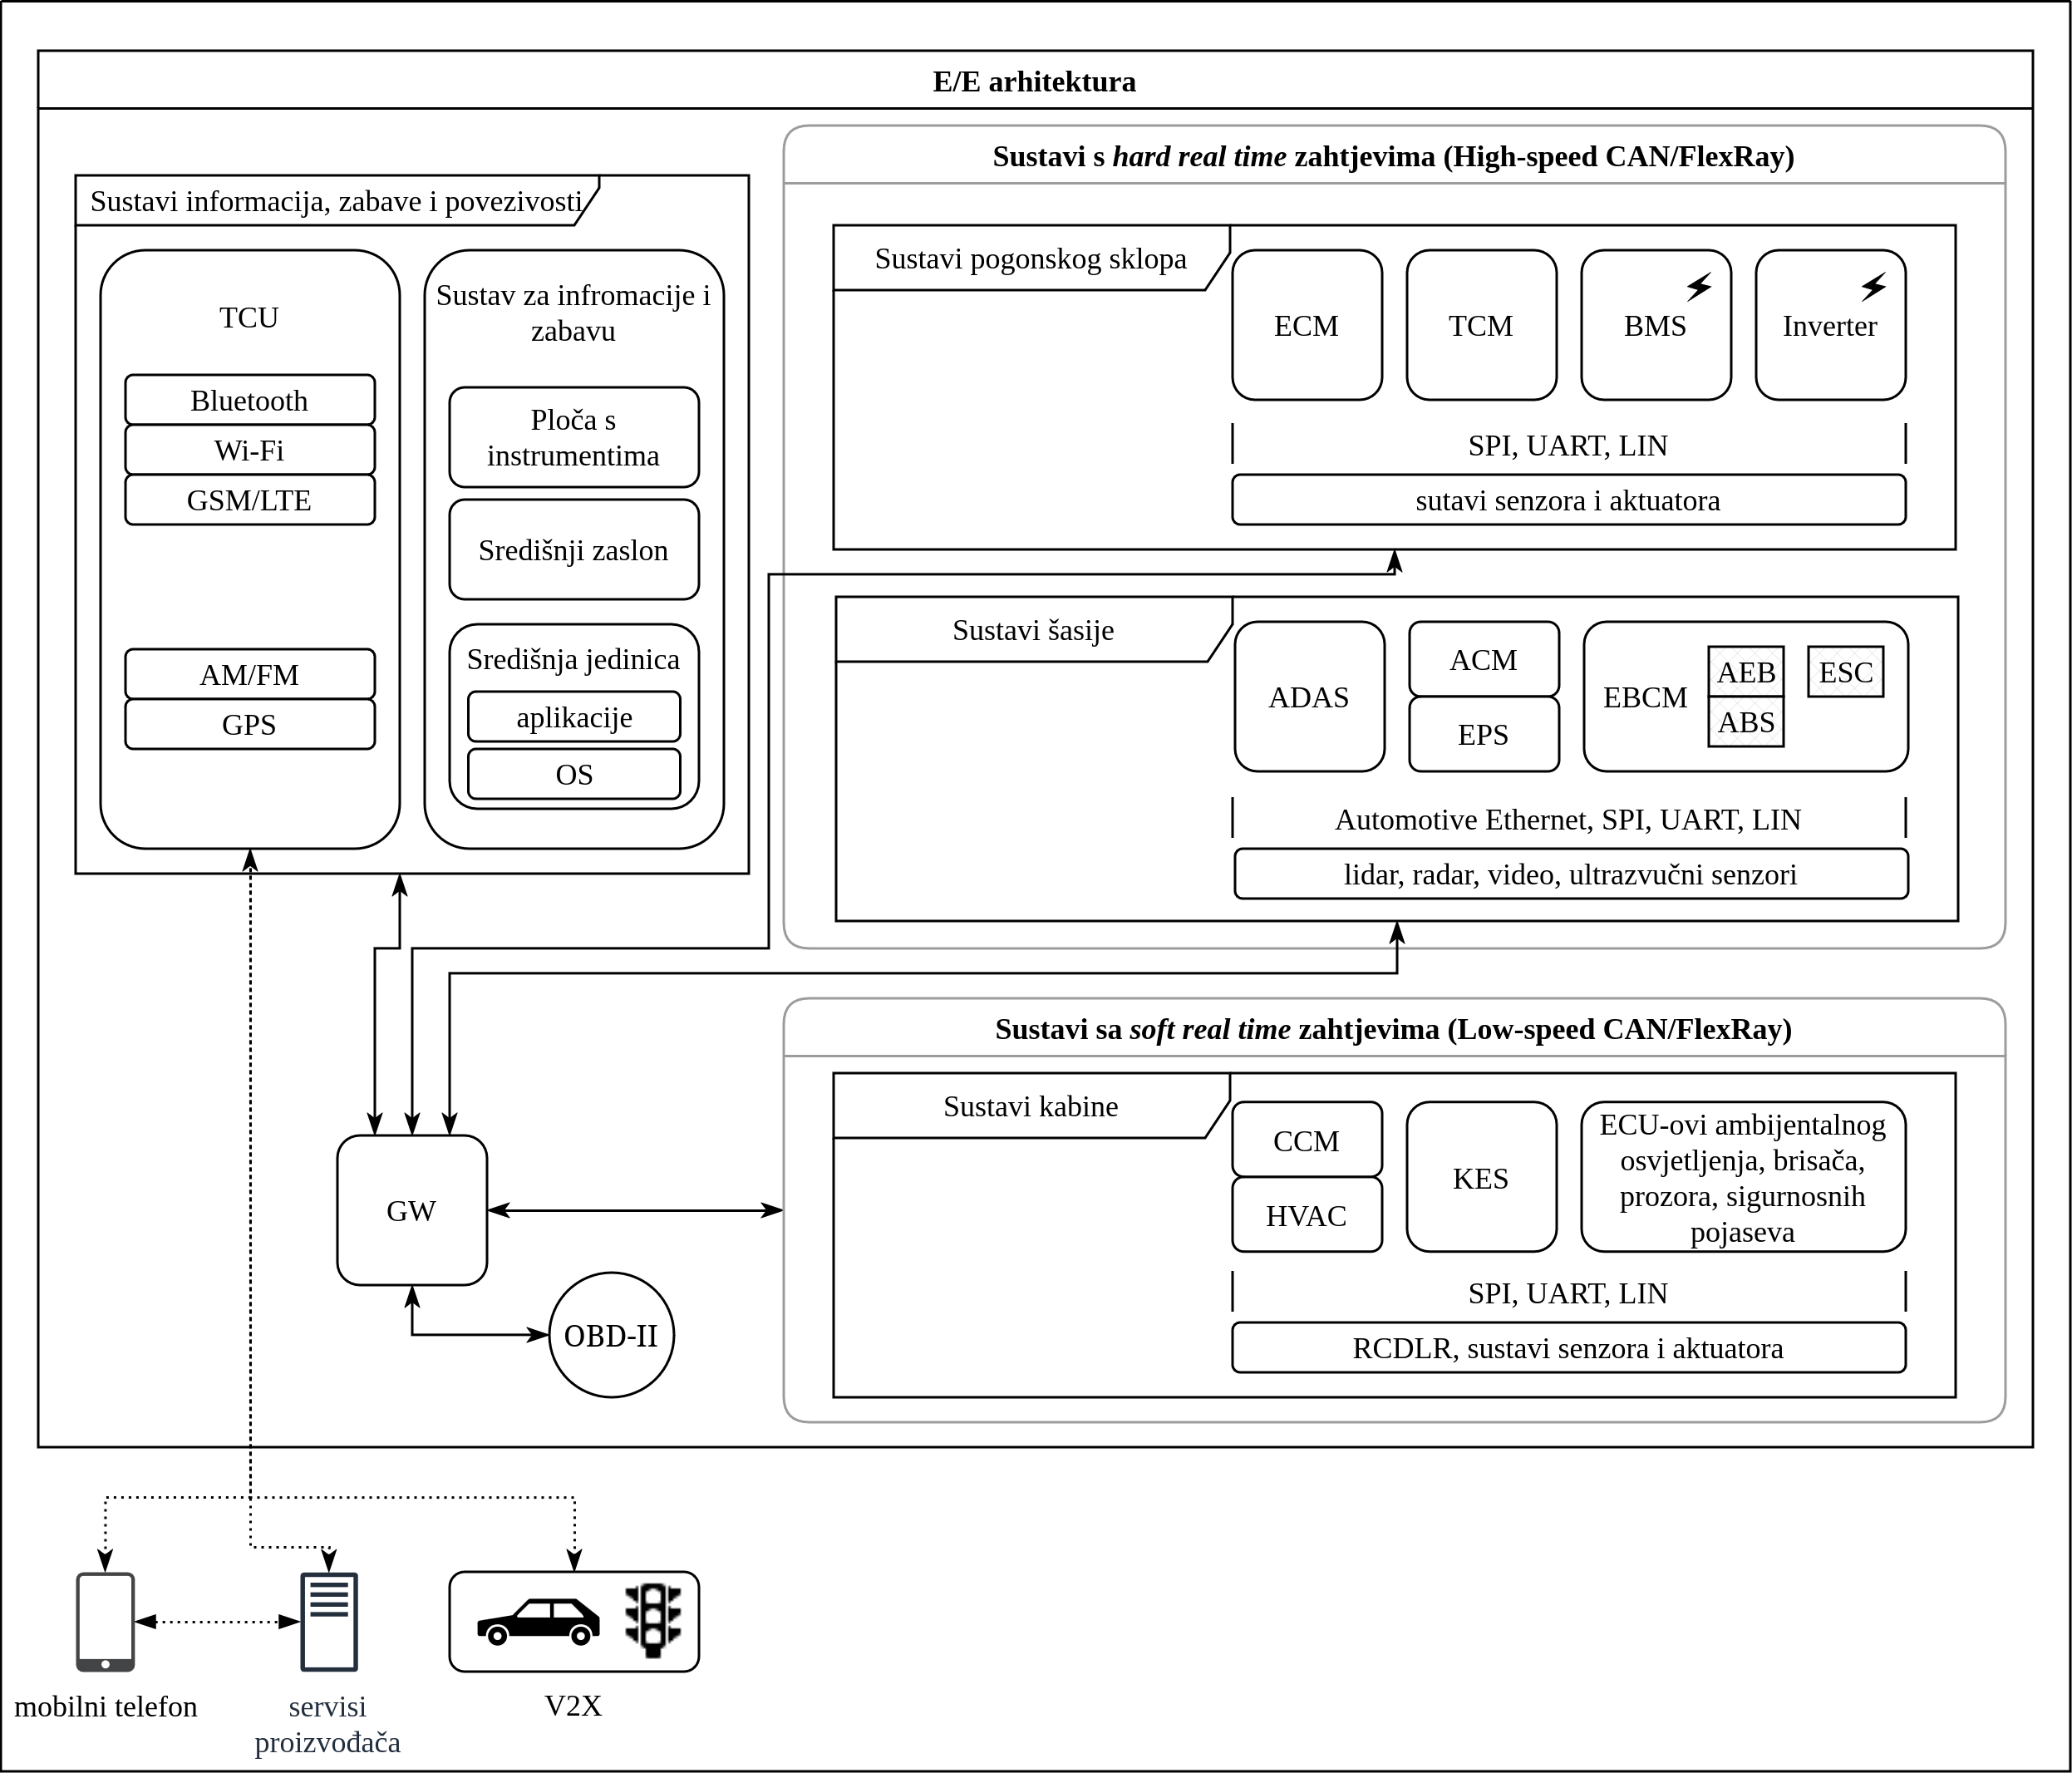
\includegraphics[width=\textwidth]{arhitektura.png}
\caption{Generalizirana arhitektura modernog automobila}
\label{fig:arhitektura}
\end{figure}
\newpage
\section{Protokoli fizičkog sloja i sloja podatkovne poveznice}
\subsection{CAN}
Protokol \textit{Controller area network} je serijski komunikacijski protokol sa svojstvima pogodnima za komunikaciju sustava u stvarnom vremenu\cite{bosch1991}. Predstavili su ga inženjeri tvrtke \textit{Robert Bosch GmbH} 1986. godine, na konferenciji \textit{Society of Automotive Engineers} (SAE) u Detroitu, a prvu primjenu u automobilskoj industriji imao je u modelu \textit{Mercedes-Benz W140}, puštenom na tržište 1991. godine te je danas standard za komunikaciju u motornim vozilima, ali se pojavljuje i u industrijskim upravljačkim sustavima\cite{bosch2022handbook, mercedes1991can}. Specifikacija CAN-a tvrtke \textit{Robert Bosch GmbH} standardizirana je u seriji standarda ISO 11898. 
\newpage
Prema \cite{bosch1991} CAN se može podijeliti u 3 sloja:
\begin{itemize}
    \item objektni sloj \engl{object layer}
    \item prijenosni sloj\engl{transfer layer}
    \item fizički sloj \engl{physical layer}
\end{itemize}
Prema OSI modelu, objektni i prijenosni sloj odgovaraju sloju podatkovne poveznice, a fizički sloj fizičkom. Objektni sloj definira filtriranje primljenih poruka te određivanje poruka koje treba prenijeti. Prijenosni sloj obuhvaća funkcije upravljanja okvirima, arbitraže, signaliziranja i provjeravanja grešaka. Fizički sloj definira kako se zapravo i kojim prijenosnim medijem signali prenose. Glavna svojstva protokola CAN su prioritizacija poruka putem nedestruktivne arbitraže, garancija vremena latencije, mogućnost postojanja više \textit{master} čvorova, detekcija i signalizacija grešaka, razlikovanje privremenih grešaka i trajnih ispada te automatsko isključivanje neispravnih čvorova. 

Na razni fizičkog sloja, razlikujemo CAN visoke brzine \engl{high-speed CAN} i CAN niske brzine \engl{low-speed CAN}, definirani u ISO 11898-2 i ISO 11898-2. CAN visoke brzine može postići brzinu prijenosa podataka do 1 Mbit/s te se koristi za komunikaciju između kritičnijih čvorova, dok je CAN niske brzine tolerantan na greške te ima maksimalnu brzinu prijenosa podataka od 125kbit/s \cite{bosch2022handbook}. Prijenosni medij je parica, koja može biti upredena ili neupredena. Podaci se šalju putem dva komplementarna signala, \textit{CAN Low} (CAN\_L) i \textit{CAN High} (CAN\_H) koji čine diferencijalni par. Razlika između napona signala CAN\_H i CAN\_L definira logičko stanje sabirnice. Diferencijalni signal čini CAN otpornijim na interferenciju, s obzirom na to da će interferencija utjecati na oba signala, ali ne i na njihovu razliku\cite{bosch2022handbook}. 

Nisko logičko stanje odnosno logička "0" je dominantno stanje, a visoko logičko stanje, logička "1", je recesivno stanje. Logička razina sabirnice u određenom trenutku može se odrediti kao logički umnožak stanja koja na sabirnicu postavljaju čvorovi u tom trenutku. Odnosno, razina sabirnice bit će u dominantnom niskom logičkom stanju u slučaju da barem jedan od čvorova postavlja dominantnu logičku "0", a u suprotnom biti će u recesivnom stanju, prikazano na primjeru s 3 čvora na slici \ref{fig:sabirnica}. 
\newpage
\begin{figure}[htb]
\centering
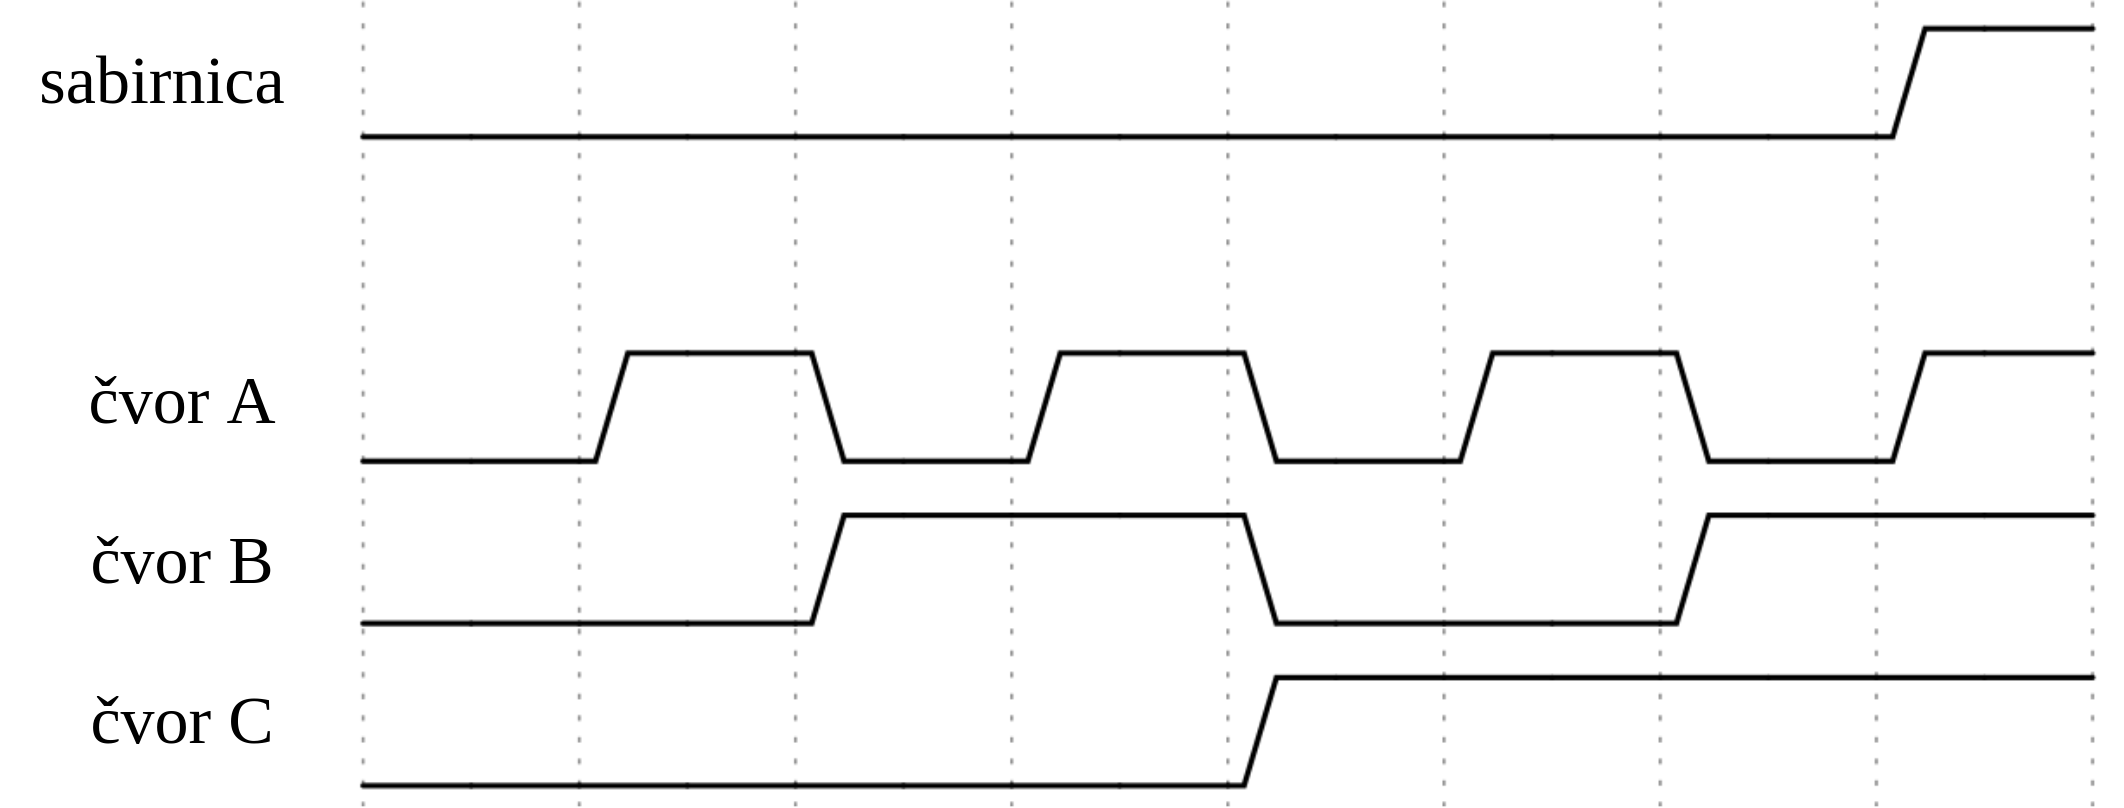
\includegraphics[width=275pt]{slike/sabirnica.png}
\caption{Logička stanja CAN sabirnice}
\label{fig:sabirnica}
\end{figure}

Opisano ponašanje omogućava sustav arbitraže i prioritizacije CAN poruka, kojim se određuje koji čvor ima prednost pri prenošenju podataka u slučaju istovremenog početka prijenosa poruka više čvorova. Svaki CAN okvir započinje bitom za početak okvira (engl. start-of-frame bit, SoF) te arbitražnog identifikatora \engl{arbitration identifier)}. Primjerice, kada dva čvora istovremeno krenu prenositi svoje poruke, odnosno prvo njihove identifikatore, oni će ih prenositi bit po bit sve dok prvi čvor ne zamijeti razliku između postavljenog i stvarnog stanja. Razlika se pojavljuje jer je drugi čvor postavio dominantnu logičku "0" kada je prvi htio postaviti recesivnu logičku "1". Nakon toga prvi čvor prepušta sabirnicu te se prebacuje u stanje čitanja, a drugi čvor prenosi svoju poruku do kraja. Nakon što sabirnica ponovno postane slobodna, prvi čvor će pokušati napraviti retransmisiju svoje poruke. Sukladno tome, poruke koje imaju manji identifikator, imaju veći prioritet, jer imaju duži neprekinuti niz nula na početku okvira. Primjer s razrješavanjem kolizije između dva čvora dalje se može proširiti na veći broj čvorova, gdje prioritet dobiva čvor čija poruka ima najmanji identifikator, a ostali čekaju završetak prijenosa. Kada se sabirnica ponovno oslobodi, ostali čvorovi započinju retransmisiju te se postupak arbitraže ponavlja.

% opis can okvira
\textit{Boschova} specifikacija inačice 2.0 CAN-a iz 1991. godine dijeli se na dijelove A i B, odnosno CAN 2.0A i CAN2.0B \cite{bosch1991}. Razlikuju se u podržanoj duljini identifikatora poruke, gdje CAN2.0B podržava standardne poruke s 11-bitnim identifikatorima i proširene poruke s 29-bitnim identifikatorima, dok CAN2.0B podržava samo standardne poruke. Razlikujemo 4 vrste CAN okvira:
\begin{itemize}
    \item podatkovni okvir \engl{data frame}
    \item okvir greške \engl{error frame}
    \item okvir zahtjeva \engl{remote frame}
    \item okvir preopterećenja \engl{overload frame}
\end{itemize}
\newpage
Glavni dijelovi podatkovnog okvira prikazanog na slici \ref{fig:CAN_okvir} su:
\begin{enumerate}
    \item bit početka okvira (engl. \textit{Start-of-Frame bit, SOF})    
    \item arbitražni identifikator \engl{arbitration ID}    
    \item bit zahtjeva za prijenosom (engl. \textit{remote transmission request}, RTR) 
    \item bit proširenja identifikatora (engl. \textit{identifier extension bit}, IDE) 
    \item kod duljine podataka {engl. \textit{data length code}, DLC}
    \item podatkovno polje        
    \item kod cikličke provjere zalihosti (engl. cyclic redundancy check)
    \item bit potvrde (\textit{acknowledge slot}, ACK)
    \item kraj okvira (engl. \textit{End-of-Frame}, EOF)        
\end{enumerate}

Uz navedene, na slici \ref{fig:CAN_okvir} pojavljuju se substitucijski bit RTR bita (engl. \textit{substitute remote request}, SSR) i bitovi r0 i r1 rezervirani za moguća proširenja protokola.
Arbitražni identifikator poruke duljine je 11 bita za standardne poruke (CAN 2.0A) i 29 bita za proširene poruke. Poruke s nižom vrijednosti identifikatora imaju veći prioritet pri arbitraži. Skupa s RTR bitom čini arbitražno polje. RTR bit u recesivnoj "1" označava okvir zahtjeva, a u dominantnoj "0" podatkovni okvir. Ovakvim označavanjem okvira postiže se prednost podatkovnog okvira pri arbitraži nad okvirom zahtjeva s istim arbitražnim identifikatorom. Za specificiranje duljine podataka u oktetima koristi se 4-bitno DLC polje od kojih se zapravo koristi 3 bita, s obzirom na to da je duljina podataka ograničena na 8 okteta. Nakon polja s podacima nalaze se CRC kod i ACK bit. Čvor koji prenosi okvir postavlja ACK bit u recesivnu "1" jer očekuje da će bar jedan čvor potvrditi ispravnost poruke postavljanjem stanja sabirnice u dominantnu "0". Naposljetku se prenosi niz od 7 recesivnih "1" kao oznaka kraja okvira (EOF).

\begin{figure}[htb]
\centering
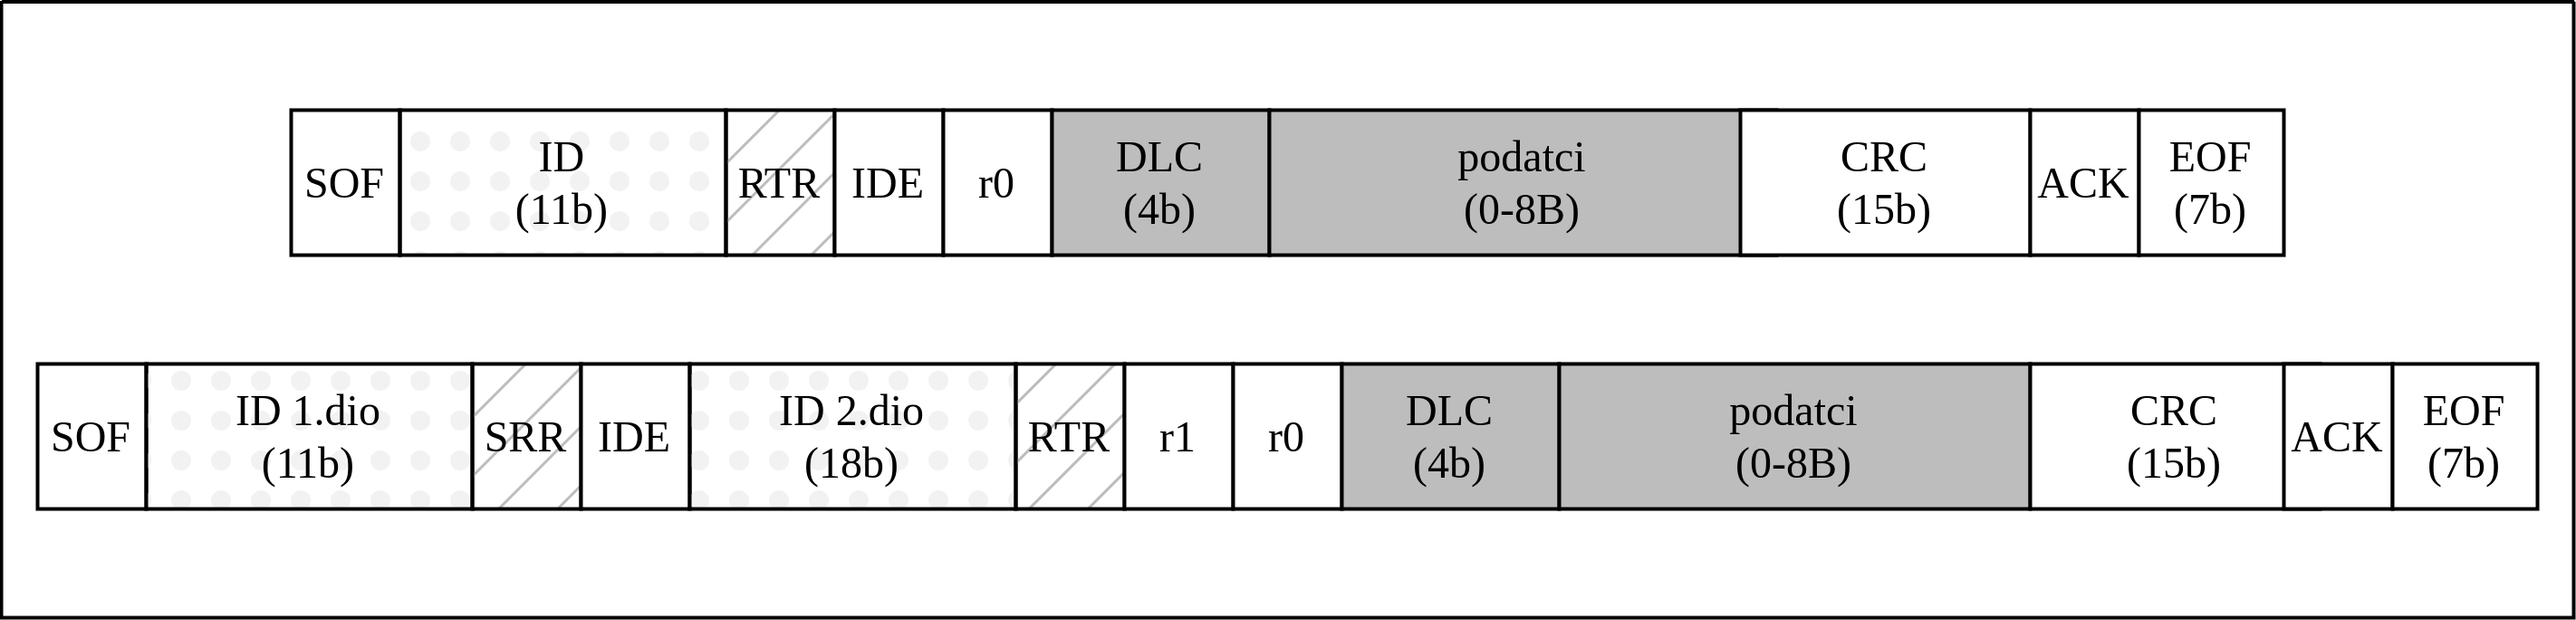
\includegraphics[width=\textwidth]{slike/CAN_okvir.png}
\caption{Standardni i prošireni CAN okvir}
\label{fig:CAN_okvir}
\end{figure}
\newpage
Prema \cite{bosch1991} CAN protokol razlikuje 5 vrsta grešaka:
\begin{itemize}
    \item greška bita \engl{bit error}
    \item greška umetnutog bita \engl{stuff error}
    \item CRC greška \engl{CRC error}
    \item greška formata \engl{form error}
    \item greška potvrde \engl{acknowledgment error}
\end{itemize}

Svaki vrsta greške od navedenih odgovara jednoj od metoda za detekciju grešaka koje su dio CAN protokola. Svaki CAN primopredajnik tijekom prijenosa poruke osluškuje sabirnicu bit po bit kako bi potvrdio da se njegova poruka ispravno prenosi. Ako se postavljeni bit i stvarni bit na sabirnici razlikuju, osim u periodu arbitraže, CAN primopredajnik će detektirati grešku bita. CAN protokol koristi i \textit{bit stuffing} metodu detekcije grešaka, odnosno umetanje dodatnog bita suprotnog polariteta nakon 5 bitova istog polariteta. Dodatne bitove uklanja primopredajnik čvora primatelja. Greškom umetnutog bita smatra se pojavljivanje 6 bita istog polariteta. Svaki čvor primatelj izračunava CRC kod primljene poruke, a razlika u izračunatom i primljenom CRC kodu smatra se CRC greškom. CAN okviri sadrže nekoliko fiksnih bitova, čija neispravnost naznačava grešku formata. Naposljetku, grešku potvrde detektira čvor pošiljatelj kada niti jedan čvor primatelj nije postavio sabirnicu u dominantnu "0" tijekom perioda ACK bita.

Svaki čvor interno održava dva brojača grešaka, brojač grešaka pri prijenosu (engl. \textit{transmit error counter}, TEC) te brojač grešaka pri primitku (engl. \textit{receive error counter}, REC). U kontekstu grešaka, čvorovi mogu biti u aktivnom, pasivnom i stanju ispada \engl{bus off}. Trenutno stanje čvora ovisi o vrijednostima TEC i REC brojača, a prijelazi su prikazani dijagramom na slici \ref{fig:error_stanja}. Kada čvor u aktivnom stanju detektira grešku postavlja aktivnu zastavicu greške u obliku 6 dominatnih bitova koji će sigurno trenutni okvir učiniti nevažećim zbog metode \textit{bit stuffing} te će ostali čvorovi u aktivnom stanju analogno reagirati postavljanjem svojih zastavica. Ovisno na kojem od 6 bitova prve zastavice ostali čvorovi detektiraju grešku, duljina cjelokupnog okvira greške može biti između 6 i 12 bitova. Čvor u pasivnom stanju u slučaju detektiranja greške postavlja pasivnu zastavicu greške u obliku 6 recesivnih bitova, u svrhu samoprovjere čvora, što može rezultirati u promjeni stanja brojača. 
\newpage
\begin{figure}[htb]
\centering
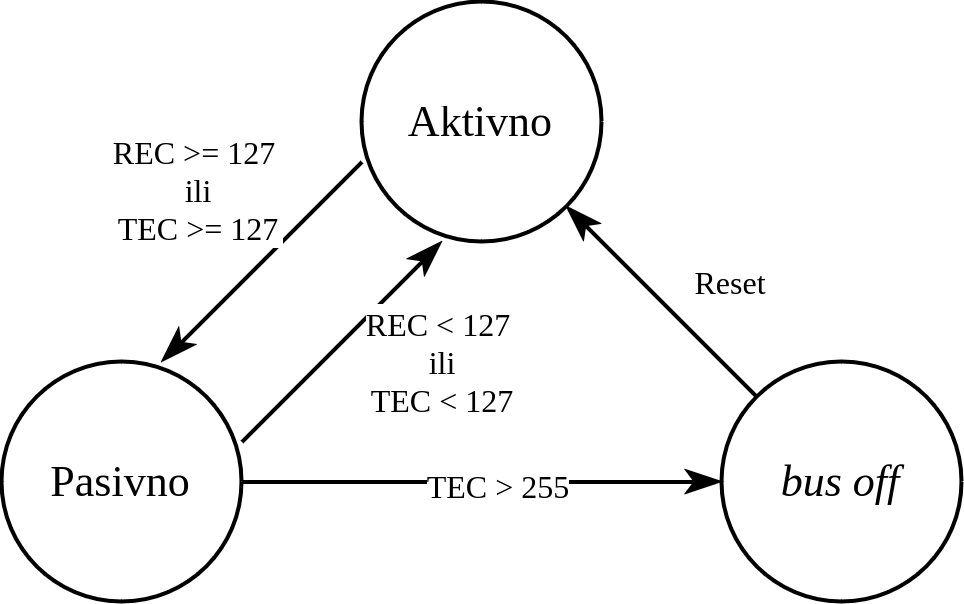
\includegraphics[width=230pt]{slike/stanja.png}
\caption{Stanja CAN čvora}
\label{fig:error_stanja}
\end{figure}

S obzirom na to da je maksimalna brzina prijenosa podataka klasičnog CAN-a 1 Mbit/s s ograničenjem od maksimalno 8 okteta podataka po poruci, tvrtka \textit{Robert Bosch GmbH} uvodi CAN s fleksibilnom brzinom prijenosa podataka (engl. \textit{CAN with Flexible Data-Rate}, CAN-FD) kao proširenje CAN-a. CAN-FD povećava maksimalnu duljinu polja podataka jednog okvira s 8 na 64 okteta. Uz navedeno, omogućava dinamično povećanje brzine prijenosa, uobičajeno do 2Mbit/s, isključivo za vrijeme trajanja prijenosa podataka nekog CAN okvira \cite{bosch2022handbook,nasser2023automotive}.

\subsection{FlexRay}
Zbog potrebe za više determinističkim komunikacijskim protokolom s garantiranom propusnosti za kritične poruke, stvoren je FlexRay \cite{nasser2023automotive}. FlexRay za razliku od CAN-a, koji koristi \textit{Code Division Multiple Access} metodu dodjeljivanja pristupa sabirnici, FlexRay koristi \textit{Time Division Multiple Access} metodu koja dodjeljuje pristup za prijenos određenih poruka po vremenskim odsječcima u dva kanala. Poruke mogu biti periodične, fiksne duljine te se za njih dodjeljuju statički vremenski odsječci ili su neperiodične, varijabilne duljine te se onda prenose u dinamičkom vremenskom odsječku \cite{nasser2023automotive}. Maksimalna duljina polja podataka jedne poruke je 254 okteta, što omogućava brzinu prijenosa podataka do 10Mbit/s u slučaju konfiguracije s jednim redundantnim kanalom. Ukoliko komunikacija nije kritična, redundantni kanal moguće je iskoristiti za udvostručenje brzine prijenosa podataka do 20Mbit/s \cite{nasser2023automotive, bosch2022handbook}. FlexRay mreže mogu biti organizirane u sabirničku topologiju ili topologiju zvijezde.
\subsection{Ethernet}
Pojava sustava s potrebama za još većom brzinom prijenosa podataka, potaknula je proizvođače na uporabu Etherneta prilagođenog za primjenu u automobilskoj industriji \engl{automotive Ethernet} u internim mrežama svojih vozila \cite{nasser2023automotive, bosch2022handbook}. Brzine prijenosa podataka kreću se u rasponu od 10Mbit/s do 10Gbit/s, što Ethernet čini priladnim za vremenski osjetljivu komunikaciju, poput spajanja domenskih upravljačkih jedinica te za primjene koje zahtjevaju veliku propusnost, primjerice prijenos video toka između ADAS-a i video senzora. Prednost korištenja Etherneta dolazi i iz kompatibilnosti s postojećim sustavima poput sigurnosnih stijena, usmjerivača te mrežnim stogovima raznih operacijskih sustava.  

Najveća prilagodbe za automobilsku industriju pojavljuju se na fizičkom sloju, koji mora biti prilagođen standardima elektromagnetske kompatibilnosti (engl. \textit{electromagnetic compatibility}, EMC).
\subsection{LIN}
\textit{Local Interconnect Network} sabirnica najčešću primjernu ima u povezivanju senzora i aktuatora s pripadajućim ECU-ovima . Primjerice, koristi se u sustavima domene šasije za upravljanje bravom vrata, podizanjem i spuštanjem prozora te namještanjem zrcala retrovizora \cite{bosch2022handbook, nasser2023automotive, dissecto2023networks}. U automobilima LIN komunikacija odvija se između \textit{master} ECU-a, koji zadaje naredbe i \textit{slave} senzora i aktuatora koji ih obrađuju i po potrebi odgovaraju. Komunikaciju pokreće \textit{master} prijenosom zaglavlja koje sadrži sinkronizacijske bitove te identifikator naredbe. \textit{Slave} odgovara prijenosom podataka maksimalne duljine 8 okteta i kontrolne sume. Iako je sporiji od CAN-a s brzinom prijenosa podataka do 20kbit/s te podržava manje fleksibilnu konfiguraciju od maksimalno 16 čvorova, prednost LIN-a je jeftin prijenosni medij u obliku jednožilnog kabela.
\section{Dijagnostički i kalibracijski protokoli}
 Dijagnostički i kalibracijski protokoli su protokoli aplikacijskog sloja OSI modela te mogu funkcionirati povrh različitih protokola nižih slojeva, ali su u ovom radu razmatrani u kontekstu CAN-a. U ovom poglavlju opisani su dijagnostički protokoli \textit{Unified Diagnostic Services} (UDS) i \textit{On Board Diagnostics II} (OBD-II) te univerzalni mjerni i kalibracijski protokol (engl. \textit{Universal Measurement and Calibration Protocol}, XCP). 
 
\subsection{Transportni protokol ISO-15765-2}
Preduvjet za ispravnu komunikaciju putem protokola UDS i OBD-II je povećanje maksimalne duljine prenesenih podataka u jednom CAN okviru. U tu svrhu, kroz standard ISO 15765, uveden je ISO-15765 transportni protokol (ISO-TP) koji omogućava pouzdan prijenos podataka veličine do 4GB povrh CAN-a ili CAN-FD-a \cite{dissecto2023isotp}. ISO-TP uvodi 6 načina adresiranja čvorova, gdje se pri korištenju normalnog načina adresiranja svakom čvoru pridjeljuju dva arbitražna identifikatora, za primanje i slanje poruka.

Podaci veći od maksimalne veličine polja podataka CAN ili CAN-FD okvira, fragmentiraju se u jedan \textit{First Frame} (FF) okvir te u više uzastopnih \textit{Consecutive Frame} (CF) okvira. Nakon FF okvira te prije primitka ostatka podataka kroz više CF okvira, primatelj mora prvo poslati \textit{Flow Control} okvir, kojim definira parametre veličine bloka i vremenskog razmaka. U slučaju da su podaci manji od maksimalne veličine polja podataka CAN ili CAN-FD okvira, prenose se \textit{Single Frame} okvirom.  

\subsection{OBD-II}
Zahtjev za uvođenjem dijagnostike u svrhu kontrole emisija u svim novim automobilima izdao je \textit{California Air Resources Board} u Kaliforniji 1991. godine. Navedena dijagnostika je nazvana \textit{On Board Diagnostics} (OBD) te je 1994. standardizirana pod nazivom OBD-II. OBD-II definira standardizirani skup dijagnostičkih informacija koje svaki ECU mora čuvati te priključak i komunikacijski protokol za pristup navedenom skupu \cite{bosch2022handbook}.

Od 2014. godine u Europskoj Uniji dozovoljeno je samo korištenje CAN-a na fizičkom sloju i sloju podatkovne poveznice te protokola ISO-TP na transportnom sloju, što je u skladu sa standardom ISO 15767 \cite{bosch2022handbook}. Međutim, priključak OBD-II uz CAN podržava i protokole \textit{Keyword Protocol 2000}, VPW i PWM te protokol standarda ISO 9141-2. Shema priključka OBD-II s označenim CAN kontaktima prikazana je na slici \ref{fig:obd2} \cite{falch2022obd}.

\begin{figure}[htb]
\centering
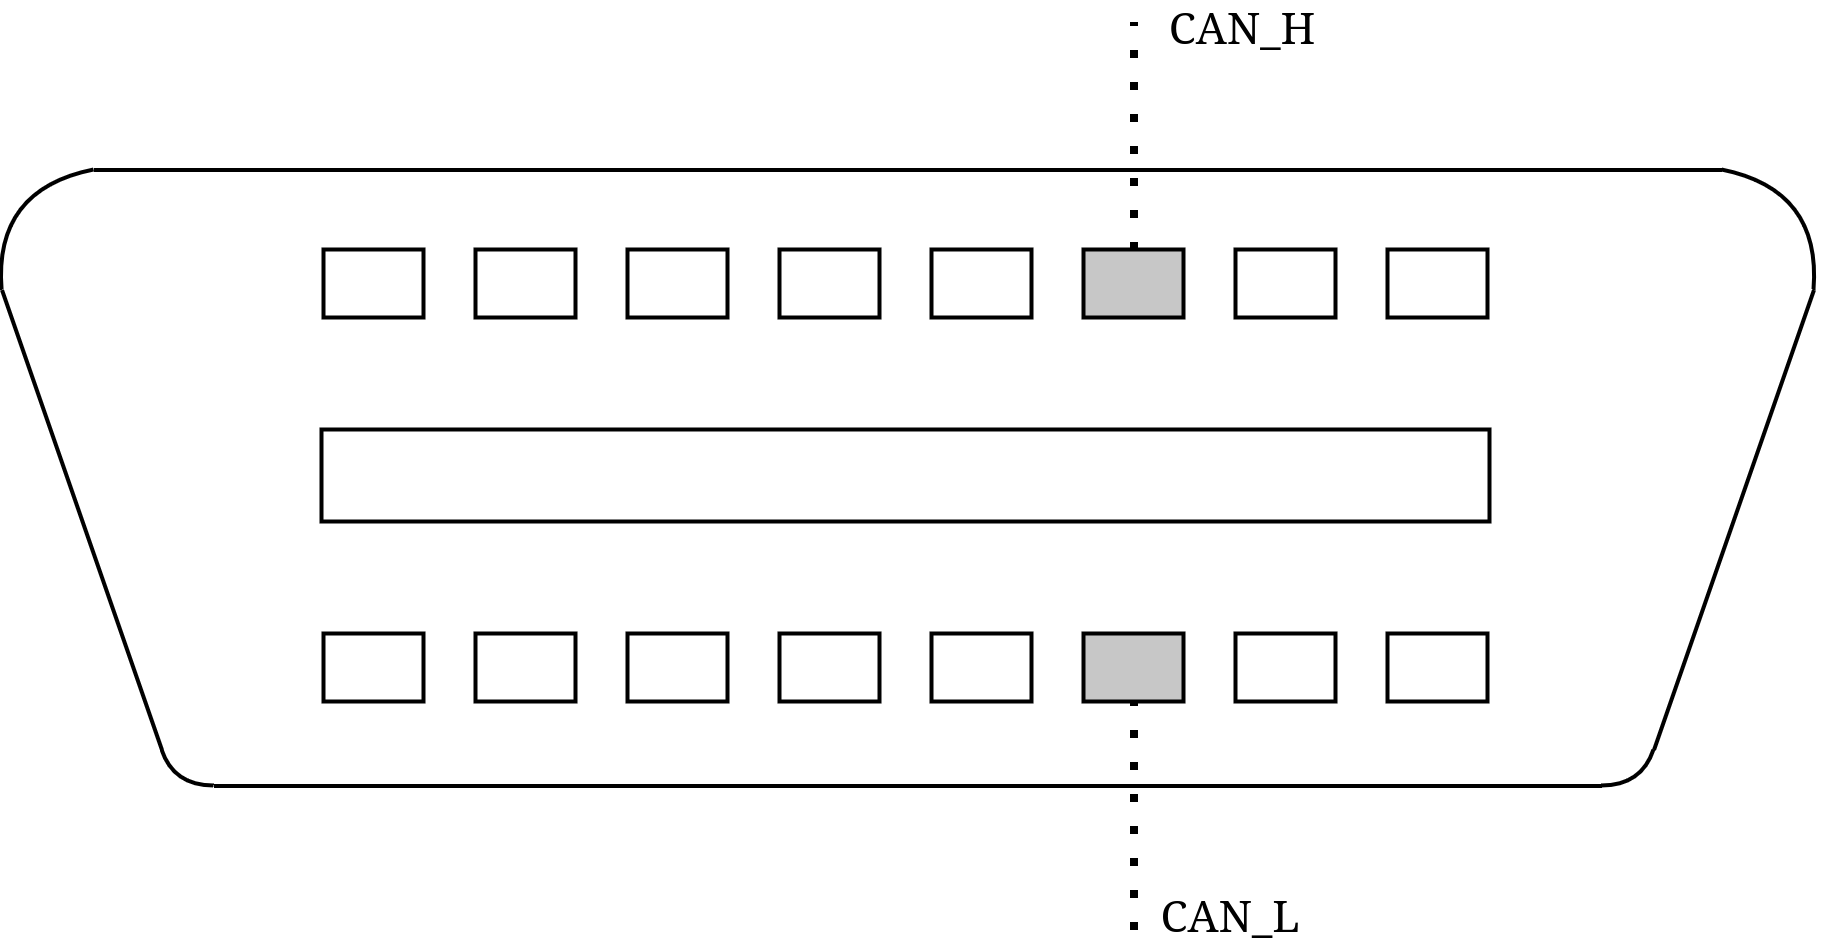
\includegraphics[width=250pt]{slike/obd2.png}
\caption{Shema OBD-II priključka}
\label{fig:obd2}
\end{figure}

Zahtjevi u protokolu OBD-II šalju se s arbitražnim identifikatorom \texttt{0x7DF}, a odgovori na zahtjeve s identifikatorima \texttt{0x7E8} do \texttt{0x7EF}. Dijagnostičke informacije poput trenutne brzine, broja okretaja te temperature motora, moguće je dohvatiti korištenjem različitih servisa s njihovim paramtarskim identifikatorima (engl. \textit{Parameter identificator}, PID). Specifičan je servis \texttt{03}, koji nudi isčitavanje dijagnostičkih kodova neispravnosti (engl. \textit{diagnostic trouble code}, DTC) te servis \texttt{04} koji omogućava njihovo brisanje \cite{falch2022xcp}.

\subsection{UDS}
\textit{Unified Diagnostic Services} (UDS) je protokol aplikacijskog sloja koji nudi niz dijagnostičkih servisa koje je moguće implementirati za pojedini ECU. Standardiziran je u ISO 14229 te povrh CAN-a koristi ISO-TP na transportnom sloju \cite{dissecto2023uds}.

ECU se u UDS komunikaciji ponaša kao poslužitelj, dok je klijent najčešće dijagnostički alat servisera ili programska podrška za konfiguraciju ECU-ova u tvornici. Kroz niz UDS servisa moguće je upravljati stanjem ili ponovno pokrenuti ECU, čitati i brisati DTC-ove, isčitavati i modificirati parametre ECU-a, testirati značajke ECU-a korištenjem ugrađenih rutina te isčitavati i modificirati sadržaj memorije, prvenstveno u svrhu ažuriranja \cite{falch2022uds}. UDS zahtjev sastoji se od identifikatora servisa (engl. \textit{service identifier}, SID), okteta podfunkcije odabranog servisa, skupa s potrebnim parametrima, prikazano na slici \ref{fig:uds}. Ukoliko je odgovor pozitivan, sadržavat će SID uvećan za 0x40 te podatke odgovora specifične tom servisu. U slučaju negativnog odogvora, odgovor počinje s oketom \texttt{0x7F} te sadrži SID zahtjevanog servisa te kod negativnog odgovora (engl. \textit{negative response code}, NRC), primjerice kod \texttt{0x11} u slučaju da ECU ne podržava zahtjevani servis. 

\bigskip
\begin{figure}[htb]
\centering
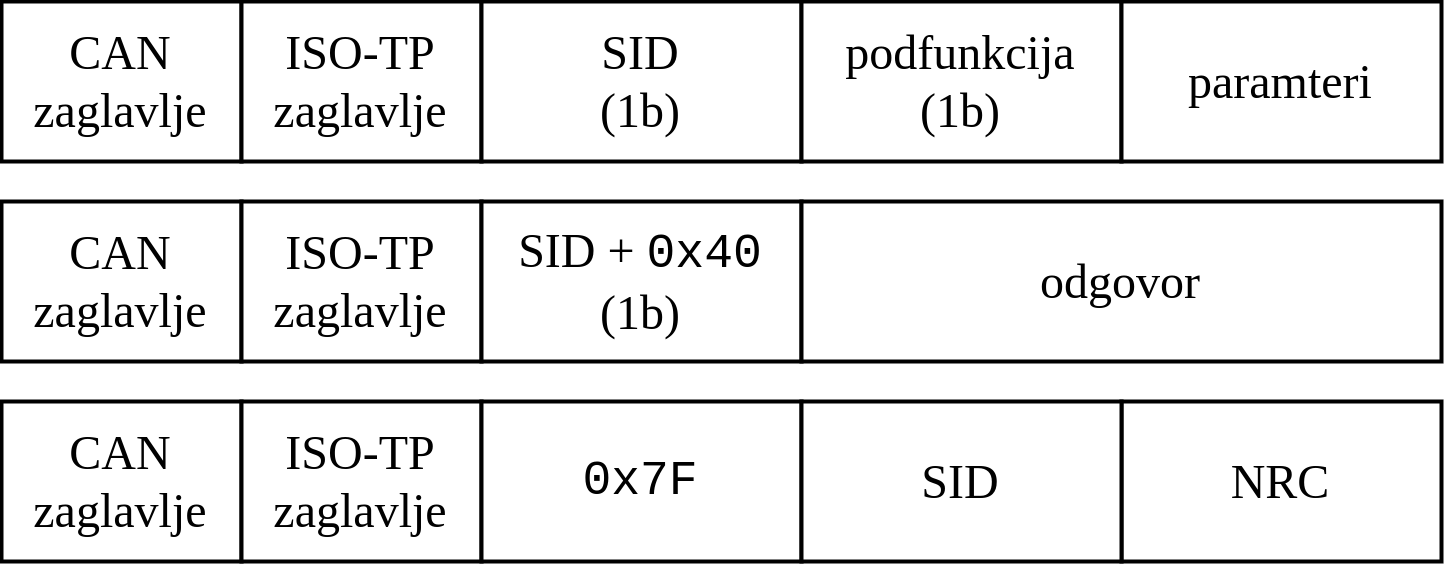
\includegraphics[width=300pt]{slike/uds.png}
\caption{UDS zahtjev, pozitivan i negativan odgovor}
\label{fig:uds}
\end{figure}

Između 27 dostupnih UDS servisa, kao sigurnosno kritične UDS servise treba izdvojiti:
\begin{itemize}
    \item \texttt{0x10 DiagnosticSessionControl}
    \item \texttt{0x11 ECUReset}
    \item \texttt{0x28 CommunicationControl}
    \bigskip
    \item \texttt{0x22 ReadDataByIdentifier}
    \item \texttt{0x23 ReadMemoryByAddress}
    \item \texttt{0x2E WriteDataByIdentifier}
    \item \texttt{0x3D WriteMemoryByAddress}
    \bigskip
    \item \texttt{0x34 RequestDownload}
    \item \texttt{0x35 RequestUpload}
    \item \texttt{0x38 RequestFileTransfer}
    \bigskip
    \item \texttt{0x2F InputOutputControlByIdentifier}
    \item \texttt{0x31 RoutineControl}
    \bigskip
    \item \texttt{0x27 SecurityAccess}
    \item \texttt{0x29 Authentication}
\end{itemize}

Servis \texttt{DiagnosticSessionControl} koristi se za izmjenu vrste dijagnostičke sesije. Dijagnostička sesija određuje kontekst izvršavanja servisa, primjerice kojem dijelu memorije se pristupa i koji dio izvršnog koda se može ažurirati. Također, servisi mogu biti podijeljeni po različitim vrstama dijagnostičkih sesija, čime se omogućava ili onemogućava njihovo korištenje. Servis \texttt{ECUReset} koristi se za pokretanje više različitih vrsta resetova ECU-ova. Vrstu reseta određuje oktet podfunkcije. Zabrana primanja i slanja poruka nekom ECU-u može se uvesti korištenjem servisa \texttt{CommunicationControl}.

Servisi \texttt{ReadDataByIdentifier} i \texttt{WriteDataByIdentifier} koriste se u svrhu čitanja i pisanja podataka spremljenima pod određenim podatkovnim identifikatorima (engl. \textit{data identifier}, DID). Značenje većine identifikatora određuje proizvođač. Za čitanje i pisanje u memoriju ECU-a koriste se servisi \texttt{ReadMemoryByAddress} i \texttt{WriteMemoryByAddress}, gdje dostupnost dijelova memorije ovisi o konkretnoj implementaciji\cite{falch2022uds, dissecto2023uds}.

Skupini servisa \texttt{0x34} do \texttt{0x38} koji služe za preuzimanje i prijenos podataka pripadaju servisi \texttt{RequestUpload}, texttt{RequestDownload} te \texttt{RequestFileTransfer}. Servisi \texttt{RequestUpload} i \texttt{RequestDownload} koriste se za započinjanje prijenosa izvršnog koda s testirane jedinice na klijenta te obrnuto. Servis \texttt{RequestFileTransfer} koristi se za preuzimanje ili prijenos datoteka te dohvaćanje informacija o datotečnom sustavu ECU-a.

Servis \texttt{InputOutputControlByIdentifier} omogućava klijentu upravljanje signalima koje ECU odašilje, njihovo zamrzavanje na trenutnoj vrijednosti ili resetiranje na pretpostavljenu vrijednost. Servis \textit{RoutineControl} omogućava klijentu aktivaciju i deaktivaciju pretprogramiranih testnih rutina te dohvaćanje njihovih rezultata.

Naposljetku, za sve UDS servise moguće je omogućiti autorizaciju ili autentifikaciju s više razina pristupa putem servisa \texttt{SecurityAccess} ili \texttt{Authentication}. Servis \texttt{0x27 SecurityAccess} koristi nespecificirani \textit{seed-and-key} algoritam. Pojam \textit{seed-and-key} upotrebljava se u UDS specifikaciji umjesto pojma izazov-odgovor \engl{challenge-response} koji je čest u ostalim granama kibernetičke sigurnosti. Slijed autorizacije servisom \texttt{0x27} može se prikazati kroz nekoliko koraka:
\begin{enumerate}
    \item Klijent šalje zahtjev za autorizacijom te dodatne parametre poput zahtjevane razine pristupa.
    \item ECU generira niz okteta \textit{seed} i šalje ga klijentu.
    \item Klijent i ECU koriste \textit{seed} kao ulaz u \textit{seed-and-key} algoritam te izračunavaju ključ.
    \item Klijent šalje \textit{seed} ECU-u.
    \item ECU uspoređuje primljeni ključ s izračunatim te odobrava ili odbija pristup klijentu.
\end{enumerate}
Sigurnost autorizacije putem servisa \texttt{SecurityAccess} ovisi o odabranom \textit{seed-and-key} algoritmu.
\newpage
Servis \texttt{Authentication} dodan je u reviziji standarda ISO-14229-1:2020 kao moderna alternativa servisu \texttt{SecurityAccess}. Temelji se na korištenju digitalnih certifikata i infrastrukture javnog ključa (engl. \textit{public key infrastructure, PKI} za autentifikaciju \cite{vector2021uds}:
\begin{enumerate}
    \item Klijent šalje zahtjev za autentifikacijom te svoj digitalni certifikat s javnim ključem.
    \item ECU verificira certifikat provjeravajući njegov potpis s javnim ključem certifikacijskog autortiteta kojem vjeruje.
    \item ECU generira niz okteta \textit{challenge} i šalje ga klijentu.
    \item Klijent izračunava digitalni potpis koristeći \textit{challenge} te svoj privatni ključ te ga šalje ECU-u.
    \item ECU verificira ispravnost potpisa koristeći javni ključ klijenta te odobrava ili odbija pristup klijentu.
\end{enumerate}

\subsection{XCP}
Protokol XCP proširenje je CAN kalibracijskog protokola (engl. \textit{CAN Calibration Protocol}, CCP) s podrškom za Ethernet, SPI, USB, FlexRay i CAN-FD kao nižim slojevima umjesto klasičnog CAN-a \cite{falch2022xcp}. Koristi se za mjerenje i kalibraciju parametara i programiranje flash memorije ECU-ova. Najčešće se koristi samo za vrijeme razvoja i testiranja ECU-a \cite{falch2022xcp}.

Komunikacija je oblika \textit{master-slave}, gdje je kalibracijski alat \textit{master}, a ECU \textit{slave}. \textit{Master} s ECU-om komunicira putem zahtjeva nazvanih \textit{Command Receive Object} (CRO) te od ECU-a dobiva \textit{Data Transmission Object} (DTO) odgovore. DTO može biti poruka odgovora na naredbu (engl. \textit{Command Response Message}, CRM), poruka događaja (engl. \textit{Event Message}, EV) te poruka dohvaćanja podataka (engl. \textit{Data Acquisition Message}, DAQ).

U slučajevima kada XCP treba ostati dostupan i nakon prodaje, moguće je kontrolirati pristup korištenjem \textit{seed-and-key} autorizacije. Za autorizaciju se koriste CRO-ovi \texttt{GET\_SEED} i \texttt{UNLOCK}, a koraci autorizacije isti su kao i kod UDS servisa \texttt{Security Access}.
\chapter{Pregled postojećih napada}
\section{Napadi specifični komunikacijskim i dijagnostičkim protokolima automobila}
opcenito opisi za ove koje ne razmatramo u detalje
\subsection{CAN}
\subsection{UDS}
\subsection{XCP}
\section{Napadi na automobile i sustave automobila}
napravi kratku analizu svega, izvuci sve napadnute sustave 
% https://illmatics.com/car_hacking.pdf
\chapter{Analiza postojećih edukacijskih materijala u području sigurnosti vozila}
hw based caputre the flag challenges,
blockharbour ctf
htb
onaj guide od valseka
... pogledaj biljeske
icsim

napravi kratku analizu svega, pokazi prednosti i nedostatke
\chapter{Implementacija sustava za obuku stručnjaka sigurnosti}

\section{Arhitektura}
\section{Zadaci}
spomeni xcp scapy ogranicenja
spomeni granicu izmedju stvari koje se prate na kontroleru i koje su na aplikacijskoj razini (TEC, busoff...)
\chapter{Zaključak}
 Zaključak.


\bibliography{literatura}
\bibliographystyle{fer}


\begin{sazetak}
Sažetak na hrvatskom jeziku.

\kljucnerijeci{Ključne riječi, odvojene zarezima.}
\end{sazetak}

% TODO: Navedite naslov na engleskom jeziku.
\engtitle{Title}
\begin{abstract}
Abstract.

\keywords{Keywords.}
\end{abstract}

\end{document}
